\section{Human-Robot Interaction} Fundamental goal of this thesis to build a systematic hand gesture recognition system to interact with machines such as robot or a computer. Interaction with them are mostly through displays, keyboards, mouse and touch interfaces. These devices have grown to be familiar but inherently limit the speed and naturalness. Previous sections have explained how we build a system to facilitate a natural interaction with the humanoid robot called NAO. Following sections illustrate how robot reacts to the hand gestures in real time with the help of Command module.

\subsection{Gesture-to-Speech} Easiest translation from the recognized hand gesture is to speak it out loud. We have used Text-To-Speech (TTS) engine that was built internally inside Aldebaran modules. When the user gesticulate the focus gesture, NAO says "WAVE" and denoting that hand tracking is started. Furthermore, the robot says words such as "Walk", "Turn Left", "Turn Right", "Move Left" and "Move Right", whenever those gestures are recognized. Additionally, it says info messages such as "Left Hand is lost", "Right Hand is lost" and "Both hands are lost" to inform the user about the internal status of hand tracking.

\subsection{Gesture-to-Motion} This thesis was initially conceived as a hand gesture translator just to say the recognized gestures loud. To make this system more useful, Gesture-to-Motion feature was added to the Command module. This functionality helps us to move the robot from one position to another in 2 dimensional space. Therefore each gesture was assigned a locomotion task as follows:

\paragraph*{Walk} This gesture commands the robot to walk in forward direction at a normalized maximum velocity (1.0) with the step frequency of 0.5. Robot walks approximately for 5 seconds and waits for the next command.

\paragraph*{Turn Left} This gesture commands the robot to rotate itself around z-axis in the left direction at a normalized maximum velocity (1.0) with the step frequency of 0.5. Robot walks approximately for 3 seconds and waits for the next command.

\paragraph*{Turn Right} This gesture commands the robot to rotate itself around z-axis in the right direction at a normalized maximum velocity (1.0) with the step frequency of 0.5. Robot walks approximately for 3 seconds and waits for the next command.

\paragraph*{Move Left} This gestures combines Walk and Turn Left by commanding the robot to rotate itself around z-axis in the left direction for 3 seconds and walk forward for 5 seconds and waits for the next command.

\paragraph*{Move Right}  This gestures combines Walk and Turn Right by commanding the robot to rotate itself around z-axis in the right direction for 3 seconds and walk forward for 5 seconds and waits for the next command.

\paragraph*{Click} This gesture is used to gain the control of the robot, when the robot lost its balance and fell down. When this gesture is executed, robot wakes up from the sleeping mode and sets itself to the standing position.

\begin{figure}	 	
	\begin{minipage}
		{.6
		\textwidth}  	
		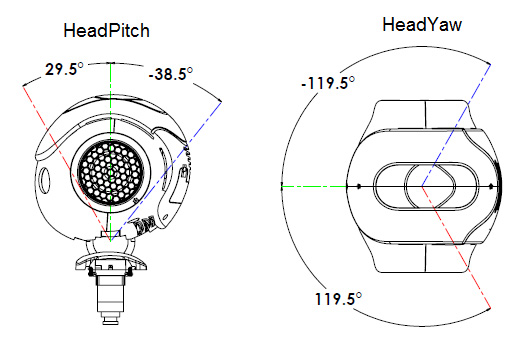
\includegraphics[height=60mm]{figures/content/nao-head.jpg} \caption{NAOs head Pitch and Yaw angle range that can be set with the help of joint control methods of NAOqi API. \cite{8} } \label{fg:nao:head} 
	\end{minipage}
	\hspace{10 mm}
	\begin{minipage}
		{.3
		\textwidth}  
		\centering
		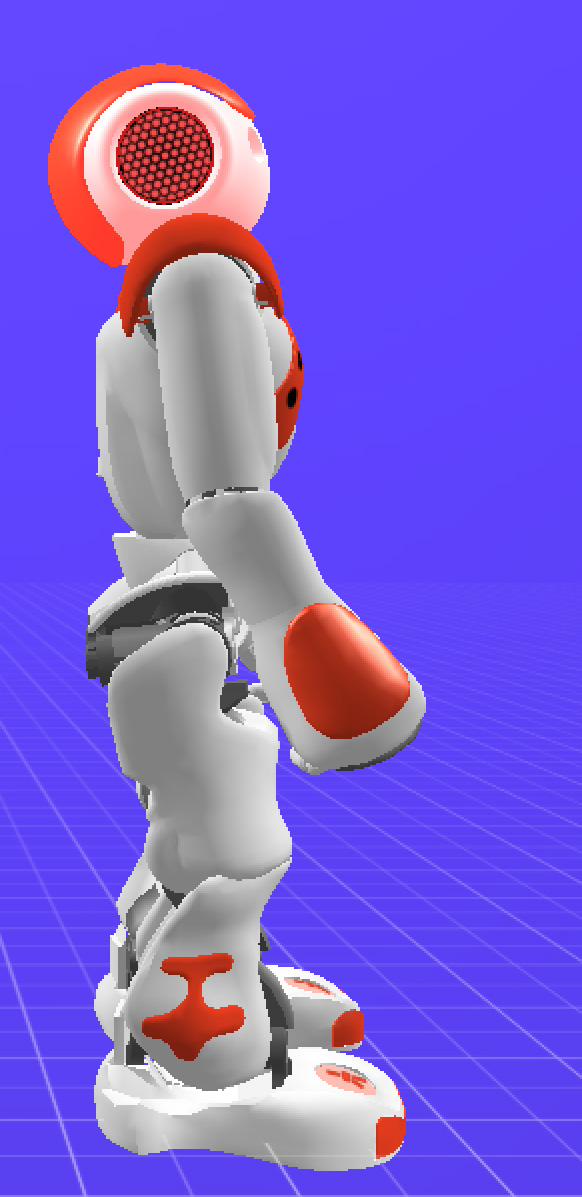
\includegraphics[height=70mm]{figures/content/nao-head-stand.jpg} \caption{Virtual NAO in Aldebaran Choregraphe with head pitch set to -18 degrees look at the upper body of the user.} \label{fg:nao:head:stand} 
	\end{minipage}	
\end{figure}




\subsubsection*{Head Position} As described in the section \ref{sec:range:train}, collection of training data for each gesture was carried out in 4 different positions in front of the robot. During this phase robot was set to standing position where the height of the robot is 58 cm. Figure \ref{fg:nao:head} shows that NAOs head can be tilted by adjusting the pitch and yaw of the head joint. In order to avoid confusing camera perspective during the training, NAOs head pitch was set to -18.0 degrees and yaw was set to 0.0 degree as shown in the figure \ref{fg:nao:head:stand}. At this angle, field of view of the depth camera was enough to cover upper body of the user. 

However, keeping the head tilted with mounted camera will cause the robot to lose balance. Therefore, NAOs head position is reset to initial stand position before it executes the received Gesture-to-Motion command. Once the locomotion phase is completed it looks back at the user. This functionality greatly improves in locating the user at any position in the Minimum-Maximum range as show in the plot \ref{pl:ges:pos}.

\subsection{Gesture-to-Gesture} Apart from offering the essential functionalities, Command module also provides Gesture-to-Gesture translation where NAO will be imitating hand gestures of the user.  Shoulder Roll and Pitch, Shoulder Roll and Yaw angles were measured by manually by positioning NAO for every gesture. When a gesture is detected, the Command modules sets the predefined angles to the shoulder and elbow joints of both the hands of NAO, therefore, translating the human hand gesture to a robotic hand gesture.

